
\subsection{Narrative as a Moat}

Hart was drawing boxes on the napkin again.

``Let’s scale this. Think beyond hedge funds. Who else needs this?''

David didn’t hesitate.  
``Anyone algorithmically allocating capital under regulatory pressure:
  Banks with quant desks;  
  Sovereign wealth arms; 
  Insurance and pensions migrating into automated trading; 
  Even crypto funds trying to look institution-grade''

Hart tapped his pen twice. ``So what’s the real market size?''

David ran the numbers aloud.

``Globally? Maybe 30{,}000 institutional allocators.  
Say 10{,}000 are actively integrating ML or automation over the next five years.  
Conservatively, 20\% are in position to buy infra — that’s 2{,}000 serious prospects.''

Hart grinned. ``Then we blitz it.''

David raised an eyebrow. ``You’re saying go wide before we even optimize?''

``Exactly,'' Hart replied. ``Control’s a second-mover problem.  
Right now, we’re building surface area. \$500K/year base. \$1 million-plus for full access: audit layer, 
traceability, and IP hooks.  
You don’t trickle this in. You carpet-bomb the category. Own the narrative before anyone else knows 
there’s a war.''

\medskip

\begin{HistoricalSidebar}{First-Mover vs. Second-Mover Advantage --- Timing the Narrative}

    The concepts of \textbf{first-mover advantage} and \textbf{second-mover advantage} are foundational 
    to modern strategic thinking in technology and finance — but their deeper implications are often 
    misunderstood.
    
    \medskip
    
    The idea of the \textbf{first-mover advantage} was popularized in the 1980s by scholars like 
    \textbf{Lieberman and Montgomery}, whose 1988 paper \textit{“First-Mover Advantages”} examined 
    the conditions under which early entrants could lock in market position through brand loyalty, 
    technological leadership, and preemption of scarce resources (Lieberman \& Montgomery, 1988).
    
    \medskip
    
    But in the same paper, Lieberman and Montgomery also highlighted a paradox: in dynamic industries, 
    being first often means bearing the cost of market education, technical bugs, and regulatory 
    friction. That’s where the \textbf{second-mover advantage} emerges — a concept refined in their 
    1998 follow-up, \textit{``First-Mover (Dis)Advantages: Retrospective and Link with the Resource-Based 
    View''} (Lieberman \& Montgomery, 1998).
    
    \medskip
    
    Here, second movers — companies that enter after the trailblazers — are able to:
  
    \medskip
  
    \begin{itemize}
        \item Learn from the mistakes of early entrants,
        \item Adopt better technology without legacy constraints,
        \item Reframe the narrative once public expectations are softened.
    \end{itemize}
    
    \medskip
    
    \textbf{Clayton Christensen}, in his influential book \textit{``The Innovator’s Dilemma''}, also 
    explored this dynamic. He showed how incumbents often fail not because they’re late, but because 
    their early advantage locks them into a mindset or architecture that becomes obsolete (Christensen, 1997). 
    Latecomers with agility — and timing — win.
    
    \medskip
    
    In Hart’s framing, the move isn’t about solving the control problem first. It’s about capturing 
    narrative real estate. Blitz first, optimize later. Stake a claim before there’s even consensus 
    that the territory exists.
    
\end{HistoricalSidebar}
  

\medskip

David scratched numbers into the corner of the napkin.

``Okay,'' he said, drawing a new box. ``Mid-curve scenario. Let’s sketch it out.''

Hart leaned forward. ``Assume traction?''

``Yeah. Let’s say we land 1,000 clients over six years,'' David said, writing it down.
``That’s hedge funds, pensions, sovereigns. We don’t need everyone. Just the serious ones.''

``What’s the average deal size?'' Hart asked.

David nodded. ``Call it \$750K per year. Some will be lower, sure, but with full integration --- 
support, usage-based scaling, enterprise terms --- it averages out.''

Hart whistled. ``That’s \$750 million in ARR.''

``Exactly,'' David said, underlining it twice. ``If retention holds, and upsell clicks, we’re talking 
\$62.5M monthly recurring by year six.''

Hart tapped the table with his pen. ``That’s a category, not a feature.''

David didn’t look up. ``That’s the goal.''

\medskip

\begin{figure}[H]
    \centering
    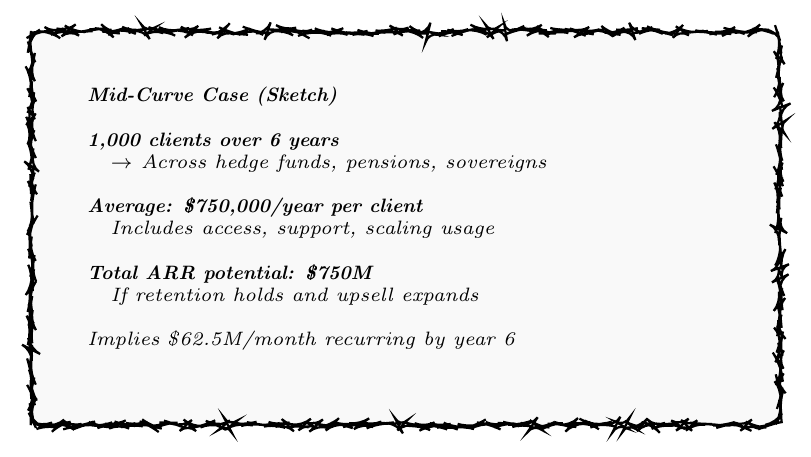
\begin{tikzpicture}[
      font=\footnotesize,
      fuzz/.style={draw=black, thick, rounded corners, fill=gray!5, decorate, decoration={random steps, segment length=2pt, amplitude=1pt}},
      txt/.style={align=left, font=\scriptsize\itshape},
    ]
  
    % Napkin box
    \node[fuzz, minimum width=9.5cm, minimum height=5cm, anchor=north west] (napkin) at (0,0) {};
  
    % Content inside
    \node[txt, anchor=north west] at ([xshift=0.6cm, yshift=-0.6cm]napkin.north west) {
      \textbf{Mid-Curve Case (Sketch)} \\
      \\
      \textbf{1{,}000 clients over 6 years} \\
      \quad $\rightarrow$ Across hedge funds, pensions, sovereigns \\
      \\
      \textbf{Average: \$750{,}000/year per client} \\
      \quad Includes access, support, scaling usage \\
      \\
      \textbf{Total ARR potential: \$750M} \\
      \quad If retention holds and upsell expands \\
      \\
      \textit{Implies \$62.5M/month recurring by year 6}
    };
  
    \end{tikzpicture}
    \caption{Napkin Sketch: Mid-curve projection for enterprise ML infrastructure revenue.}
\end{figure}

\medskip

\begin{TechnicalSidebar}{What is ARR and Why Does It Matter?}

    \textbf{ARR}, or \textit{Annual Recurring Revenue}, is a core metric for evaluating the health and scalability of 
    a subscription-based business.  
    It answers one question: \textbf{If we changed nothing, how much revenue would we make next year?}
    
    \medskip
    
    Unlike one-time sales or services, ARR assumes continuity — customers staying onboard, renewals flowing in, and 
    contracts holding steady (Bain \& Company, 2020).  
    This makes it a preferred benchmark for investors, especially in enterprise SaaS, infrastructure, and 
    fintech platforms (Benaroya \& Tan, 2022).
    
    \medskip
    
    \textbf{Why do investors care?}
  
    \medskip
    
    \begin{itemize}
      \item \textbf{Predictability:} ARR provides visibility into future cash flows (Graham, 2020).
      \item \textbf{Scalability:} High ARR growth often implies network effects or strong product-market fit (Ghosh, 2019).
      \item \textbf{Valuation:} Many high-growth companies are valued as a multiple of ARR, not EBITDA or profit 
      (Tzuo \& Weisert, 2018).
    \end{itemize}
    
    \medskip
    
    \textbf{Here's a back-of-envelope example:}  
    1,000 clients paying \$750K/year = \$750 million ARR.  
    If we assume a 10x revenue multiple then we get a \$7.5B potential valuation.
    
    \medskip
    
    \textit{In short: ARR is more than just a finance number.}  
    It’s the story of future certainty, told in dollars per year.
    
\end{TechnicalSidebar}
  

\medskip

They had moved to the bar by then. The dinner plates were cleared. Hart’s jacket was off, his sleeves pushed up, and the 
lights had dimmed just enough to signal that the crowd was thinning, but not enough to end the night.

A jazz trio murmured in the corner. Ice clinked in lowball glasses. David swirled his scotch, letting the silence stretch 
before continuing.

\medskip

``And that’s just the base stack,'' Morales said, gesturing with his glass.  
``We can spin out modules like data engines, stress frameworks, and volatility overlays.  
Each one’s a license vector. Or an acquisition target.''

Hart nodded slowly, scribbling something onto a cocktail napkin.

``At a 10x revenue multiple, that’s a \$7.5 billion ceiling.''

He looked up. ``But that’s not the point.  
The point is to scale past everyone’s comfort zone — fast enough that no one catches up.''

David leaned back, watching the amber catch in the bar light.

``You won’t get there by pitching dashboards,'' he said.  
``You need belief. You need momentum. And you need a fear of missing out.''

Hart raised his glass, smiling. ``Exactly. Blitz the market. Control the myth.''

David tapped his glass gently against Hart’s. ``You won’t get there without narrative control.''

``That’s why we’re building the narrative ourselves,'' Hart said, and drank.


\medskip

\begin{HistoricalSidebar}{The Blitzscaling Playbook: Growth First, Friction Later}

    The term \textbf{blitzscaling} was popularized by LinkedIn founder Reid Hoffman and entrepreneur Chris Yeh in their 
    2018 book of the same name (Hoffman \& Yeh, 2018).  
    It describes the strategy of prioritizing \textbf{rapid scaling over efficiency}: deliberately accepting chaos, instability, 
    and short-term loss in pursuit of long-term dominance.
    
    \medskip
    
    \textbf{The idea?} In winner-take-most markets (especially network-based or tech-driven), the biggest risk isn’t 
    inefficiency. The biggest risk is irrelevance (Hoffman \& Yeh, 2018; Eisenmann, 2013).  
  
    \medskip
  
    The first company to reach critical scale locks in network effects, captures users, and scares off late-stage capital 
    for competitors (Moazed \& Johnson, 2016).
    
    \medskip
    
    These are the core blitzscaling tactics:
  
    \medskip
    
    \begin{itemize}
      \item \textbf{Ignore traditional management advice.} Scale even when systems aren’t ready.
      \item \textbf{Outspend competitors.} Win land grabs before profit matters.
      \item \textbf{Hire ahead of revenue.} Prioritize coverage and speed over org clarity.
      \item \textbf{Fundraise fast and frequently.} Capital becomes both fuel and moat.
    \end{itemize}
    
    \medskip
    
    Consider the case of AirBnB.
  
    \medskip
    
    In 2011–2013, AirBnB was losing money in most markets. Its customer service operations were 
    overwhelmed, and regulators were circling (Gallagher, 2017). However, its leadership doubled down on blitzscaling:
    
    \begin{itemize}
      \item Rapid geographic expansion to dozens of cities per quarter.
      \item Aggressive marketing with subsidized travel, and referral programs.
      \item Growing headcount, scaling trust \& safety, increasing support, and engineering all at once.
    \end{itemize}
    
    \medskip
    
    The result?
  
    \medskip
    
    \begin{itemize}
      \item In 2011: Airbnb was valued at \$1B.
      \item By 2014: \$10B.
      \item And by IPO in 2020: over \$100B (Soper \& Chapman, 2020).
    \end{itemize}
    
    \medskip
    
    Blitzscaling worked, but it wasn't without cost:  
    Legal battles, housing backlash, employee burnout, and early investor dilution were all part of the path (Guttentag, 2015).
    
    \medskip
    
    \textbf{The takeaway?}  
    Blitzscaling is a bet that \textit{dominance now} is worth \textit{disarray today}.  
    It’s not for every company. However, in capital-rich, timing-sensitive markets, it can be the difference between first place 
    and forgotten.
    
  \end{HistoricalSidebar}
  
